\chapter{Informacje o autorze}\label{chap:cv}

\section*{Dane osobowe}

\phantom a

\noindent
\begin{tabular}{p{12cm}c}
\vspace{0.7cm}
\textbf{Andrzej Więckowski}\\[0.5ex]
witryna domowa: \href{https://andywiecko.github.io}{\normalsize\texttt{andywiecko.github.io}}\\[0.5ex]
\textsf{ORCID}: \href{https://orcid.org/0000-0002-8113-4021}{\normalsize\texttt{0000-0002-8113-4021}}\\[0.5ex]
Google Scholar user: \href{https://scholar.google.com/citations?user=X9qrSQoAAAAJ}{\normalsize\texttt{X9qrSQoAAAAJ}}
\end{tabular}

\vspace{-0.2cm}
\mymarginpar{\footnotesize
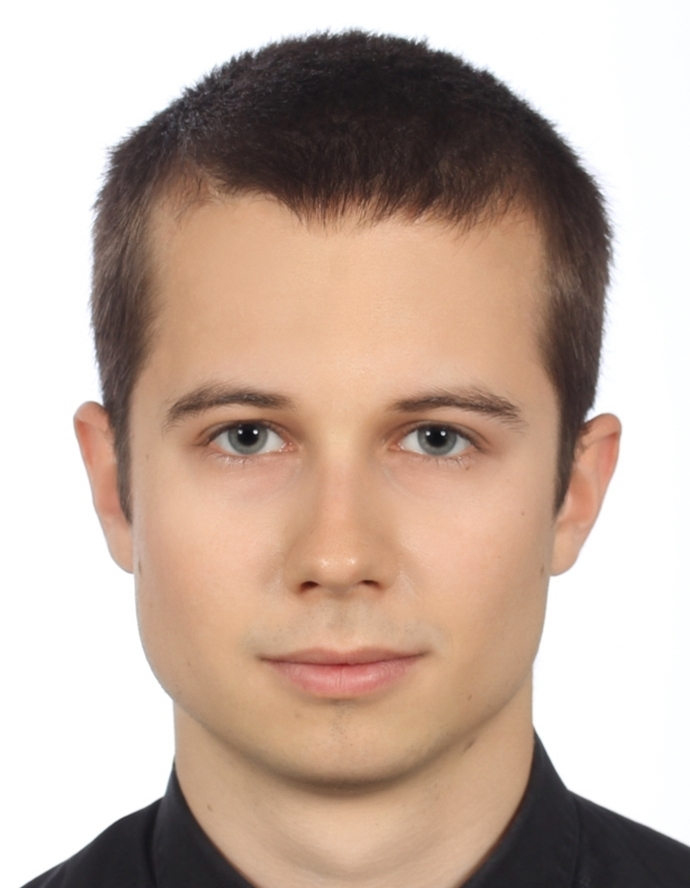
\includegraphics[width=0.7\marginparwidth]{04-Includes/Figures/photo.jpg}
%\captionof{figure}{ Ettore Majorana, niezły dzik}
} 

\vspace{0.3cm}

\ornament

\section*{Edukacja}


\phantom a

\vspace{-2.1ex}

\noindent
\begin{tabular}{p{12cm}c}
\textbf{Politechnika Wrocławska} & \textbf{2018--2020} \\[1ex]
Studia trzeciego stopnia, nauki fizyczne,\\ promotor: prof. dr hab. Marcin Mierzejewski\\[3ex]
\textbf{Uniwersytet Śląski w Katowicach} & \textbf{2013--2018}\\[1ex]
\textbf{Praca magisterska} & 2018\\
\href{https://andywiecko.github.io/assets/msc_thesis.pdf}{\textit{Dynamics of disordered quantum annealers}},\\ obroniona z wyróżnieniem, promotor: prof. dr hab. Marcin Mierzejewski\\[1ex]
Studia drugiego stopnia, fizyka: theoretical physics, & 2016--2018 \\
promotor: prof. dr hab. Marcin Mierzejewski\\[1ex]
\textbf{Praca inżynierska} &  2016\\
\href{https://andywiecko.github.io/assets/beng_thesis.pdf}{\textit{Numeryczne metody analizy dynamiki nanodrutów kwantowych}},\\ obroniona z wyróżnieniem, promotor: Prof. dr hab. Marcin Mierzejewski\\[1ex]
Studia pierwszego stopnia,  międzywydziałowe indywidualne studia matematyczno przyrodnicze, kierunki: informatyka i fizyka techniczna,\\ opiekun: dr hab. inż. Michał Mierzwa  & 2013--2016 \\
\end{tabular}

\ornament

\newpage
 
\section*{Publikacje} 
\subsection*{Rozprawa doktorska}

\phantom a
\vspace{-10ex}

\begin{enumerate}

\item A. Więckowski, M. Mierzejewski, M. Kupczyński,
    Majorana phase gate based on thegeometric phase,
    \href{http://dx.doi.org/10.1103/PhysRevB.101.014504}{\textsw{Phys. Rev. B}},
    \href{http://dx.doi.org/10.1103/PhysRevB.101.014504}{101:014504} (2020);

\item  A. Więckowski, A. Ptok, Influence of long-range interaction on Majorana zero modes, \href{https://journals.aps.org/prb/abstract/10.1103/PhysRevB.100.144510}{\textsw{Phys. Rev. B} 100, 144510} (2019);

\item A. Więckowski, M.M. Maśka, M. Mierzejewski, Majorana modes in interacting systems identified by searching for local integrals of motion, 
\href{https://journals.aps.org/prl/abstract/10.1103/PhysRevLett.120.040504}{\textsw{Phys. Rev. Lett.} 120, 040504} (2018);

\end{enumerate}
\subsection*{Praca magisterska}

\phantom a
\vspace{-5ex}

\begin{enumerate}
\setcounter{enumi}{3}

\item  A. Więckowski, S. Deffner, B. Gardas, Disorder-assisted graph coloring on quantum annealers, \href{https://journals.aps.org/pra/abstract/10.1103/PhysRevA.100.062304}{\textsw{Phys. Rev. A} 100, 062304} (2019);


\end{enumerate}


\subsection*{Pozostałe}

\phantom a
\vspace{-5ex}

\begin{enumerate}

\setcounter{enumi}{4}

\item  K. Jałowiecki, A. Więckowski, P. Gawron, B. Gardas, Parallel in time dynamics with quantum annealers, \href{https://arxiv.org/pdf/1909.04929.pdf}{arXiv:1909.04929}, w recenzji;

\item  A. Więckowski, A. Ptok, Dynamics of quantum annealers – Ising model with transverse field study, w recenzji;

\item A. Więckowski, \textsw{Proceedings of the silesian cross-border workshop on applied physics}, Majorana states in the Kitaev model with many-body interactions, ISBN: 978-80-248-3974-5 (2016).
\end{enumerate}

\ornament

\section*{Granty}

\begin{tabular}{p{12cm}c}
Wykonawca grantu 2016/23/B/ST3/00647 \textit{Dynamika niejednorodnych układów kwantowych z oddziaływaniami wielociałowymi}. & 2018--2020
\end{tabular}

\ornament

\vspace{-0.1cm}

\section*{Ważniejsze konferencje naukowe}

\phantom a
\vspace{-5ex}

\begin{itemize}
\item Mini-symposium on: Recent developments in the theory of topological systems, Lublin, Poland, 2019;

\item XIX National Conference on Superconductivity, Bronisławów, Poland, 2019;

\item Adiabatic Quantum Computing Conference, Innsbruck, Austria, 2019;

\item Majorana modes and beyond, MagTop, Warsaw, Poland, 2019;

\item 42th International conference of theoretical physics: ’Correlations and coherence at different scales’, Ustroń, Poland, 2018;

\item 26th International Conference on Atomic Physics: Summer School, Barcelona, Spain, 2018;

\item XVIII National Conference on Superconductivity, Krynica Morska, Poland, 2017;

\item Silesian cross-border workshop on applied physics, Ostrave, Czech Republic, 2016;

\item 40th International conference of theoretical physics: ’Correlations and coherence at different scales’, Ustroń, Poland, 2016.
\end{itemize}

\ornament